\documentclass[a4paper,portrait,columns=2]{cheatsheet}
\usepackage{graphicx}
\usepackage{tikz}
\usetikzlibrary{positioning}

\title{Probability and Statistics}
\author{Matthew Scicluna\\\href{mailto:matthew.scicluna@umontreal.ca}{matthew.scicluna@umontreal.ca}}
\begin{document}

%\maketitle


\section{Probability Vs Statistics}
\textbf{Probability}: Given Model, how likely is Data? $\rightarrow$ Well-formed since these are Mathematical questions.\\
\textbf{Statistics}: Given Data, how likely is Model? $\rightarrow$ Ill-formed since many Models can create the same data!

\begin{center}
	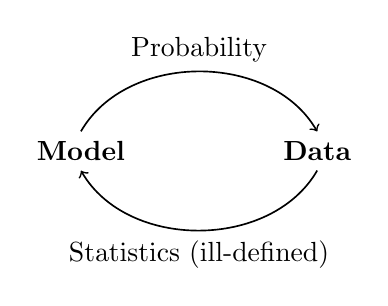
\begin{tikzpicture}[-latex, auto, node distance = 3cm and 3cm, on grid, semithick,
	state/.style ={circle, top color = white, draw, text = black, minimum width=2.5cm}]
	\node (A) {\textbf{Model}};
	\node (B) [right = of A] {\textbf{Data}};
	
	\draw [->, out=60, in=120] (A.north) to node[above]{Probability}  (B.north);
	\draw [->, out=-120, in=-60] (B.south) to node[below]{Statistics (ill-defined)} (A.south);
	\end{tikzpicture}
\end{center}

\section{Probability Space}
\textbf{Probability Space}: a triple \( (\Omega, F, P)\) consisting of:
\begin{enumerate}
	\item \( \Omega \) the \textbf{Sample Space}
	\item \( F \subseteq 2^{\Omega}\) a \textbf{\(\sigma\)-algebra} on \(\Omega\) i.e.
	\begin{enumerate}
		\item \(\Omega \in F\)
		\item \(E \in F \Rightarrow E^{\complement} \in F\)
		\item \(E_1, E_2, \cdots \in F \Rightarrow\bigcup_{i=1}^{\infty} E_i \in F\)
	\end{enumerate}
	\item \(P\): \(F \mapsto [0,1] \) a \textbf{Probability Measure} i.e.
	\begin{enumerate}
		\item \(P(E) \ge 0\) for \(E \in F\)
		\item \(P(\Omega) = 1\)
		\item \(P \left(\bigsqcup_{i=1}^{\infty} E_i \right)\Rightarrow\sum_{i=1}^{\infty} P(E_i)\) for \(E_i \in F\)
	\end{enumerate}
\end{enumerate}

Given \textbf{Events} \(E_i, E \in F\), $P$ also satisfies:
\begin{enumerate}
\item \textbf{Upward and Downward continuity} of \(P\):
	\begin{enumerate}
	\item \(E_i \uparrow E \Rightarrow \lim\limits_{n\to\infty} P(E_n) = P(E) \)
	\item \(E_i \downarrow E \Rightarrow \lim\limits_{n\to\infty} P(E_n) = P(E) \)
	\end{enumerate}
\item \textbf{Monotonicity} of \(P\):
        \begin{enumerate}
        	\item \( E_i \subseteq E_j \Rightarrow P(E_i) \le P(E_j)\)
        \end{enumerate}
\end{enumerate}

\section{Conditional Probability}
We can compute Probabilities of Events Conditioned on other Events. \\
\textbf{Conditional Probability} of event \(A\) on event \(B\) with \(P(B) > 0\) is:
\begin{align*}
P(A \mid B) = \frac{P(A \cap B)}{P(B)} = \frac{P(B \mid A)P(A)}{P(B)}
\end{align*}

A set of events \(\{A_i\}\) are \textbf{Mutually Independent} if, for any n element subset of \(\{A_i\}\):
\begin{align*}
P \left( \bigcap_{i=1}^{n} A_i \right) = \prod_{i=1}^{n}P(A_i) 
\end{align*}

\textbf{Law of Total Probability}: Given Events \(A\) and \textbf{Partition} \(\{B_i\}\) (i.e. where \(\bigsqcup_{i=1}^{\infty} B_i = \Omega \) )
\begin{align*}
P(A) = \sum_{i=1}^{\infty} P(A \mid B_i)P(B_i)
\end{align*}



\section{Random Variables}

A \textbf{Random Variable} is a \(\mathbb{B}\)-Measurable function \\
X: \( (\Omega, F) \mapsto (\mathbb{R},\mathbb{B}) \)
\begin{enumerate}
	\item For \( A \in \mathbb{B}\) we can compute \( P(X \in A)\)
	\item \( P(X \in A) := P(X^{-1}(A)) = P(\{ \omega \in \Omega : X(\omega) \in A \})\)
	\item \( P(X^{-1}(\cdot)) := P_X(\cdot)\) which is called the \textbf{Push-Forward Measure} of \(P\) by \(X\) on \( \mathbb{R}\)
	\item Hence \( X\) induces a new Probability Space \((\mathbb{R}, \mathbb{B}, P_X) \) from the original \( (\Omega, F, P)\)
\end{enumerate}

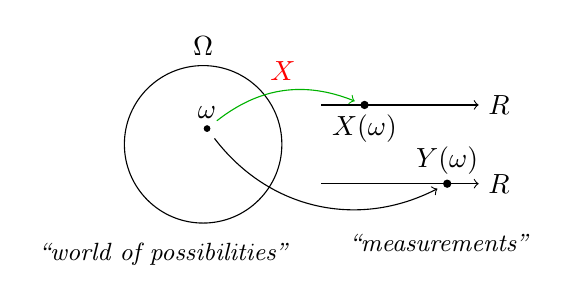
\begin{tikzpicture}[scale=0.5]
%% \draw[help lines] (0,0) grid (12,6);
%% \node [align=center, red] at (1, 1.5) {bla \\ bla} ;
%% \draw [blue, thick] (6,5) rectangle (10,10);
\draw (0,0) circle (2cm);
\node[above] at (0,2) {$\Omega$};
\node (o) at (0.1,.4) {};
\draw (o) circle[radius=2pt] node[above] {$\omega$};
\fill (o) circle[radius=2pt];
\node at (-1,-2.8) {\emph{\small ``world of possibilities''}};

\draw [->] (3,1) -- (7,1) node[right]{$\mathbb{R}$};
\node (x) at (4.1,1) {};
\draw (x) circle[radius=2pt] node[below] {$X(\omega)$};
\fill (x) circle[radius=3pt];
\draw [->, green!70!black] (o) to [bend left=30] node[midway, above, red] {$X$} (x);

\draw [->] (3,-1) -- (7,-1) node[right]{$\mathbb{R}$};
\node (y) at (6.2,-1) {};
\draw (y) circle[radius=2pt] node[above] {$Y(\omega)$};
\fill (y) circle[radius=3pt];
\draw [->, thin] (o) to [bend right=40] (y);
\node at (6,-2.5) {\emph{\small ``measurements''}};
\end{tikzpicture}

Random Variables can be uniquely determined by their \textbf{CDF}:
\( F_X(t) := P_X\left((-\infty,t]\right) = P(X \le t) \)
\begin{enumerate}
	\item Right Continuous
	\item Non-Negative
	\item \(\lim\limits_{t \to \infty} F_X(t) = 1, \lim\limits_{t \to -\infty} F_X(t) = 0\)
	\item Any function satisfying above properties is the CDF for some random variable.
\end{enumerate}

Random Variables studied are usually either \textbf{Continuous} or \textbf{Discrete} (although they can be neither.)
\begin{enumerate}
	\item If \( F_X\) \textbf{Absolutely Continuous} then \(X\) is Continuous.
	\begin{enumerate}
		\item \textbf{Absolutely Continuous}: $F$ differentiable a.e. and $\exists f(x)$ s.t. $F_X(x) = \int_{-\infty}^{x} f(u) du$
		\item \(f\) is called the \textbf{PDF}
		\item Where $f$ is continuous, $\frac{d}{dx}F_X(x) = f(x)$
		\item hence, $f$ is unique a.e. (may not be everywhere!)
		\item If \(X\) also Non-Negative then \textbf{Hazard} of X is \( \lambda(t) = \frac{f(t)}{1 - F(t)}\)	
		\begin{enumerate}
			\item \(1 - F(t) = \exp\left(-\int_0^t \lambda(x)\,dx \right) \)
			\item \(\lambda(t)\) interpreted as instantaneous survival rate at time t.
			\item \( \lambda(t) = c \ \forall t \iff X \sim Exp(c) \)
		\end{enumerate}
	\end{enumerate}
	\item If \(Range(X)\) is countable then \(X\) is Discrete.
	\begin{enumerate}
		\item \(f(x):=P(\{X=x\})\)
	\end{enumerate}
\end{enumerate}

\section{Random Vectors}
\textbf{Joint CDF} for \( \vec{X} = (X_1, X_2, ..., X_n)\) is \(F(t_1,...,t_n)=P(X_1 \le t_1, ..., X_n \le t_n)\)
\begin{enumerate}
	\item  \textbf{Marginal PDF} of \(\vec{X}_{1:p} = (X_{1}, \cdots X_{p})\) is 
	\begin{align*}
	f_{\vec{X}_{1:p}}\left(\vec{u}_{1:p}\right) = \int_{\vec{X}_{(p+1):n}}f_{\vec{X}}\left(\vec{u}_{1:p}, \vec{X}_{(p+1):n}\right)d\vec{X}_{(p+1):n}
	\end{align*}
	\item \textbf{Conditional PDF} on \(\vec{X}_{1:p}\) given \(\vec{X}_{(p+1):n}\) is 
	\begin{align*}
	f_{\vec{X}_{1:p} | \vec{X}_{(p+1):n}}\left(\vec{u}_{1:p}, \vec{u}_{(p+1):n}\right) =\frac{f_{\vec{X}}\left(\vec{u}_{1:p}, \vec{u}_{(p+1):n}\right)}{f_{\vec{X}_{(p+1):n}}\left(\vec{u}_{(p+1):n}\right)}
	\end{align*}
	\item \textbf{kth Order Statistic} \( X_{(k)}\) of \( \vec{X}\) is the kth smallest value
	\begin{enumerate}
		 \item \( f_{X_{(1)}}(u) = \sum_{i=1}^n f_{X_i}(u)\prod_{j \ne i}(1 - F_{X_j}(u))\)
		\item \( f_{X_{(n)}}(u)=\sum_{i=1}^n f_{X_i}(u)\prod_{j \ne i}F_{X_j}(u)\)
	\end{enumerate}
\end{enumerate}


\section{Moments of a Random Variable}
\(\mathbb{E}_X(X^r) := \mathbb{E}(X^r)\) is the \textbf{\(r\)th Moment} of \(X\) under the distribution of \(X\)
\begin{enumerate}
	\item \(\mathbb{E}(X) = \int_0^\infty 1 - F_X(t)\,dt - \int_{-\infty}^0 F_X(t)\,dt\)
	\item If \(X\) Continuous, \(\mathbb{E}(X) = \int_{-\infty}^{\infty} t \cdot f_X(t)\,dt\)
	\item \textbf{LOTUS}: \(\mathbb{E}(g(X)) = \int_{-\infty}^{\infty} g(t) \cdot f_X(t)\,dt\)
\end{enumerate}
Can generate Moments using the \textbf{MGF} of \(X\): \( M_X(t) = \mathbb{E} \left(\exp(Xt) \right) \), if \( \exists \epsilon >0 \) s.t. \( \forall |t| < \epsilon\),  \(M_X(t) < \infty \)
\begin{enumerate}
	\item \( \exists \epsilon >0 \) s.t. \( \forall |t| < \epsilon\),  \(M_X(t) = M_Y(t) \Rightarrow X\) and \(Y\) have same distribution
	\item \(\mathbb{E}(|X^r|) = \left.\frac{\partial^r}{\partial^r t}M_X(t)\right\rvert_{t=0}\), if \(M_X\) exists.
	\item If \(\{ X_i\}\) independent RVs, then \( M_{\sum X_i} (t) = \prod M_{X_i}(t)\)
	\item Moments most commonly analyzed are:
	\begin{enumerate}
		\item \textbf{Mean} of \(X\): \(\mathbb{E}(X):=\mu_X\)
		\item \textbf{Variance} of \(X\): \(Var(X)=\mathbb{E}((X-\mu_{X})^2)=\sigma^2_{X}\)
	\end{enumerate}
\end{enumerate}
If \(X\) and \(Y\) are Random Variables on the same Probability Space
\begin{enumerate}
	\item \textbf{Law of Total Expectation}: If \(\mathbb{E}(|X|)<\infty\) \(\mathbb{E}(X)=\mathbb{E}_{Y}(\mathbb{E}_{X \mid Y}(X \mid Y))\)
	\item \textbf{Law of Total Variance}: If \(Var(X)<\infty\)
	\(Var(X)=\mathbb{E}(Var(X \mid Y))+Var(\mathbb{E}(X \mid Y))\)

\end{enumerate}

For random vectors we have

\section{Notes}
\begin{enumerate}
	\item Continuity of \(X\) as a function has nothing to do with its continuity as a Random Variable (which depends on the absolute continuity of its CDF) \cite{976739}

	\item \(\mathbb{E}(|X|)<\infty\) iff \(\mathbb{E}(X)\) exists, by the definition of lebesgue integrability and the measurability of \(X\)
	
	\item 
	
\end{enumerate}

\newpage

\bibliography{prob_cs}
\bibliographystyle{ieeetr}



\end{document}